\documentclass[tikz]{standalone}
\usepackage{tikz}
\usepackage{amssymb}
\usetikzlibrary{positioning}
\newcommand{\MonetaryLevel}{Monetary level}
\newcommand{\RealLevel}{Real level}
\newcommand{\Firms}{Firms}
\newcommand{\Households}{Households}
\newcommand{\Banks}{Banks}
\newcommand{\Commodities}{Commodities}
\newcommand{\LaborPower}{Labor power}
\newcommand{\Wages}{Wages}
\newcommand{\Consumption}{Consumption}
\newcommand{\Credits}{Credits}
\newcommand{\Withdrawals}{Withdrawals}
\newcommand{\Deposits}{Deposits}
\newcommand{\Repayments}{Repayments}
\usetikzlibrary{arrows.meta}

\newcommand{\yslant}{0.6}
\newcommand{\xslant}{-0.8}
\usetikzlibrary{calc,intersections,arrows.meta}
\usepackage{tikz-3dplot}

\begin{document}
	
	
	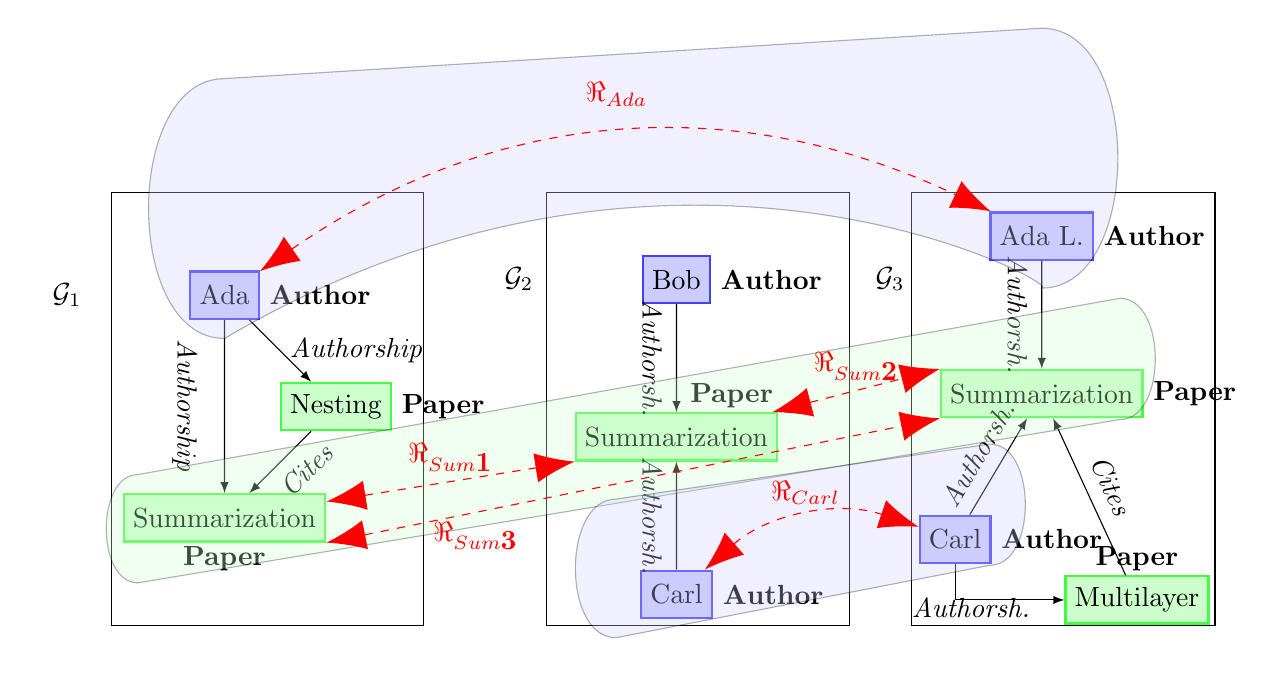
\begin{tikzpicture}[scale=1.1,every node/.style={minimum size=1cm,node distance=2cm},on grid]
	
	
	\tikzstyle{place}=[circle,thick,draw=blue!75,fill=blue!20,minimum size=6mm]
	\tikzstyle{red place}=[place,draw=red!75,fill=red!20]
	\tikzstyle{green place}=[place,draw=green!75,fill=green!20]
	\tikzstyle{transition}=[rectangle,thick,draw=black!75,
	fill=black!20,minimum size=4mm]
	
	\begin{scope}[
	xshift=0
	]
		\draw[black, thin] (-1.3,-2) rectangle (2.3,3); 
		
		\node  (w1) {};
		\node [place,rectangle] (ada1) [above of=w1,label=right:\textbf{Author}] {Ada};
		\node [left of=ada1] {$\mathcal G_1$};
		\node [green place,rectangle] (nest) [below right of=ada1,label=right:\textbf{Paper}] {Nesting};
		\node [green place,rectangle] (sum1) [below left of=nest,label={[label distance=-0.3cm]below:{\textbf{Paper}}}] {Summarization};
		\node at ($(sum1)+(0,.5)$) (g) {};
		\draw[-latex] (ada1) -- (nest) node [right,midway] {\textit{Authorship}};
		\draw[-latex] (ada1) -- (sum1) node [near end, midway,sloped,below] {\textit{Authorship}};
		\draw[latex-] (sum1) -- (nest) node [midway,below,sloped,yshift=.2cm] {\quad\textit{Cites}};
	\end{scope} 		
	
	\begin{scope}[
	xshift=120
	]
		\draw[black, thin] (-0.5,-2) rectangle (3,3); 
		
		% Agents:
		\node [place,rectangle] at (1,2) (bob) [label=right:\textbf{Author}] {Bob};
		\node [left of=bob] {$\mathcal G_2$};
		\node [green place,rectangle] (sum2) [below of=bob,label={[label distance=-.3cm,xshift=.7cm]above:{\textbf{Paper}}}] {Summarization};
		\node [place,rectangle] (carl) [below of=sum2,label=right:\textbf{Author}] {Carl};
		\draw[-latex] (bob) -- (sum2) node [near end, midway,sloped,below,yshift=.2cm] {\textit{Authorsh.}};
		\draw[-latex] (carl) -- (sum2) node [near end, midway,sloped,below,yshift=.2cm] {\textit{Authorsh.}};
	\end{scope} 
	
	\begin{scope}[
	xshift=240
	]
		\draw[black, thin] (-0.5,-2) rectangle (3,3); 
		\node at (-0.75,2) {$\mathcal G_3$};
		% Agents:
		\node [place,rectangle] at (1,2.5) (ada2) [label=right:\textbf{Author}] {Ada L.};
		\node [green place,rectangle] (sum3) [below of=ada2,label=right:{\textbf{Paper}}] {Summarization};
		\node [place,rectangle] at (0,-1) (carl2) [label=right:\textbf{Author}] {Carl};
		\node [green place,rectangle] at (2.1,-1.7) (multi) [label={[label distance=-0.3cm]above:{\textbf{Paper}}}] {Multilayer};
		\draw[-latex] (ada2) -- (sum3) node [near end, midway,sloped,below,yshift=.2cm] {\textit{Authorsh.}};
		\draw[-latex] (carl2) -- (sum3) node [near end, midway,sloped,above,yshift=-.2cm] {\textit{Authorsh.}};
		\draw[-latex] (multi) -- (sum3) node [near end, midway,sloped,above,yshift=-.2cm] {\textit{Cites}};
		\draw[-latex] (carl2) |- (multi) node [near end, midway,sloped,below,yshift=.4cm,xshift=.2cm] {\textit{Authorsh.}};
	\end{scope} 
	
	
	\filldraw[fill=green!20,opacity=.3] ($(sum1)+(-1,0.5)$) 
	--
	($(sum3)+(0.9,1.1)$) 
	to[out=0,in=0] 	  
	($(sum3)+(0.9,-0.3)$) 
	--
	($(sum1)+(-1,-0.75)$)
	to[out=180,in=180] 
	($(sum1)+(-1,0.5)$);
	
	\draw[{Latex[length=5mm]}-{Latex[length=5mm]},dashed,color=red] (sum1) edge node [midway,above,yshift=-.2cm] {$\Re_{Sum\textbf{1}}$} (sum2.south west);
	\draw[{Latex[length=5mm]}-{Latex[length=5mm]},dashed,color=red] (sum2) edge node [midway,above,yshift=-.2cm] {$\Re_{Sum\textbf{2}}$} (sum3.north west);
	\draw[{Latex[length=5mm]}-{Latex[length=5mm]},dashed,color=red] (sum1.south east) -- (sum3.south west) node[midway, below,xshift=-2cm,yshift=-.2cm] {$\Re_{Sum\textbf{3}}$};
	
	\filldraw[fill=blue!20,opacity=.3] ($(ada1)+(-0,2.5)$) 
											--
										($(ada2)+(0,2.4)$) 
											to[out=0,in=0] 	  
										($(ada2)+(0,-0.6)$) 
											.. controls ($(ada2)+(0.3,-0.6)$) and ($(bob)+(0,2.4)$) ..  
										($(ada1)+(-0,-0.5)$)
											to[out=180,in=180] 
										($(ada1)+(-0,2.5)$);
										
	\draw[{Latex[length=5mm]}-{Latex[length=5mm]},dashed,color=red] (ada1) edge [bend left] node [midway, above] {$\Re_{Ada}$} (ada2);

	\filldraw[fill=blue!20,opacity=.3] ($(carl)+(-0.7,1.1)$) 
	--
	($(carl2)+(0.4,1.1)$) 
	to[out=0,in=0] 	  
	($(carl2)+(0.4,-0.3)$) 
	--
	($(carl)+(-0.7,-0.5)$)
	to[out=180,in=180] 
	($(carl)+(-0.7,1.1)$);
	\draw[{Latex[length=5mm]}-{Latex[length=5mm]},dashed,color=red] (carl) edge [bend left] node [midway, above,yshift=-0.2cm] {$\Re_{Carl}$} (carl2);
	
	
	\end{tikzpicture}
\end{document}
